\begin{mdframed}[style=warning]
	\begin{ejercicio}
		\textbf{Conceptos.}
		\begin{enumerate}
			\item Si $\vec{A}$ y $\vec{B}$ son vectores distintos de cero, ¿es posible que $\vec{A} \cdot \vec{B}$ y $\vec{A} \cp \vec{B}$? Explique.
			\item Muestre que sin importar lo que sean $\vec{A}$ y $\vec{B}$, $\vec{A} \cdot \qty(\vec{A} \cp \vec{B}) = 0$.
		\end{enumerate}
	\end{ejercicio}
\end{mdframed}









\begin{mdframed}[style=warning]
	\begin{ejercicio}
		Dados los vectores $\vec{A}$ y $\vec{B}$, con un ángulo $\theta$ entre ellos demuestre, utilizando el producto punto, que la magnitud del vector resultante $\vec{R}$ de la suma $\vec{A} + \vec{B}$ es
			$$ R = \sqrt{A^2 + B^2 + 2AB\cos{\theta}} $$
		donde $A$ y $B$ son las magnitudes $\vec{A}$ y $\vec{B}$.
	\end{ejercicio}
\end{mdframed}







\begin{mdframed}[style=warning]
	\begin{ejercicio}
		\begin{itemize}
			\item Encuentre el ángulo entre las diagonales de las caras contigüas de un cubo.
			\item Encuentre el ángulo mostrado en la figura.
			\begin{figure}[H]
				\centering
				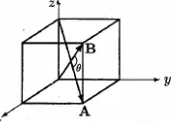
\includegraphics[scale=0.5]{./img/cube.png}
			\end{figure}
		\end{itemize}
	\end{ejercicio}
\end{mdframed}






\begin{mdframed}[style=warning]
	\begin{ejercicio}
		\begin{multicols}{2}
		Utilice el producto cruz para encontrar las componentes del vector unitario $\vu{n}$ perpendicular a una de las caras del tetraedro de la siguiente figura:
		\columnbreak
		\begin{figure}[H]
			\centering
			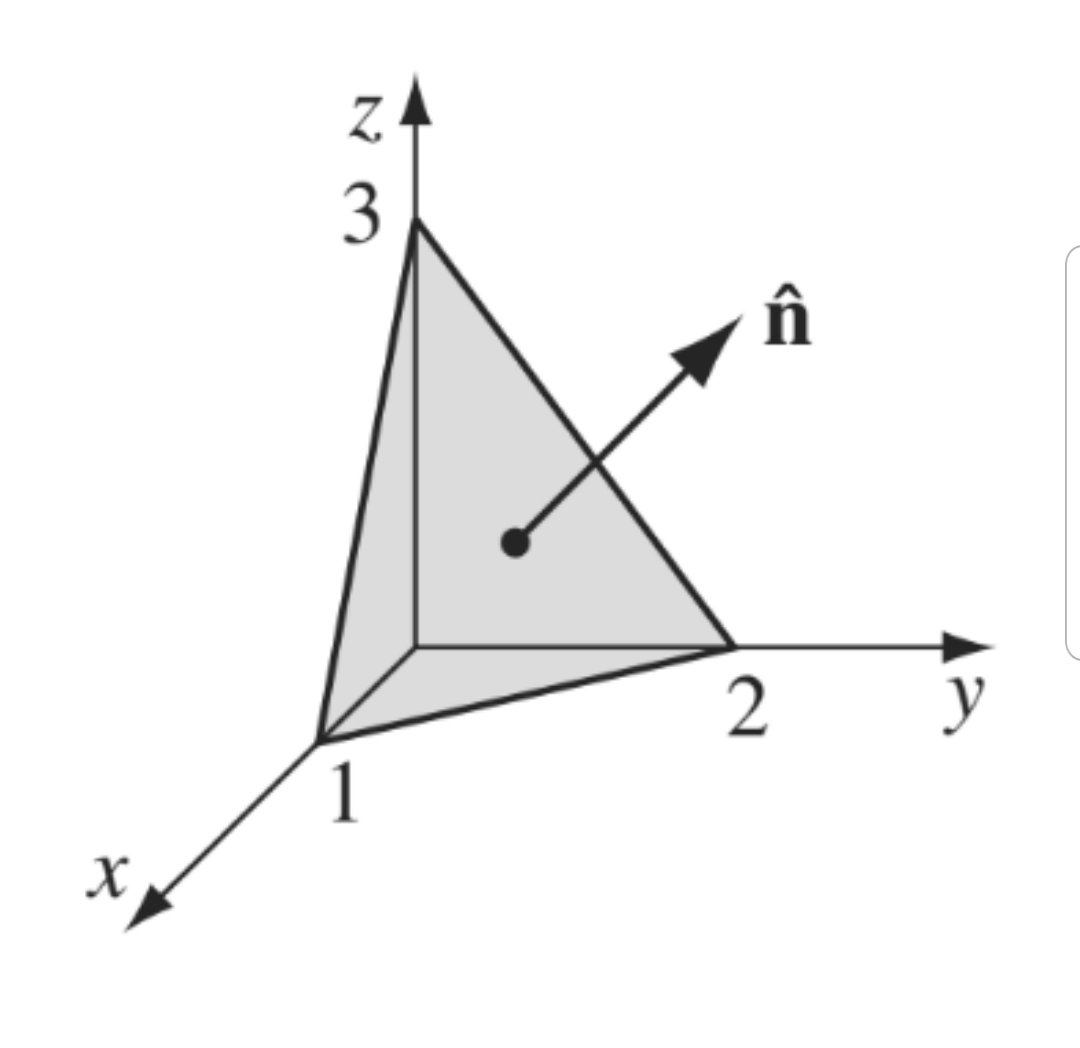
\includegraphics[scale=0.07]{./img/tetraedro.jpeg}
			\caption{Tetraedro.}
			\label{tetraedro}
		\end{figure}
		\end{multicols}
	\end{ejercicio}
\end{mdframed}

















































%%%